
\section{Server-Konfiguration}
Für dieses System wird einerseits ein \ac{DBMS} benötigt. Anderseits ist ein \textbf{MQTT-Broker} erforderlich, um die Daten vom ESP32 zu bekommen. In diesem System wird als Server ein \ac{RasPi} verwendet. Um es einfacher zu machen, werden für alle Passwörter die Zeichenkombination \textbf{''Kennwort1''} verwendet. Für den Benutzernamen wird ein sinnvoller Name gewählt, der zur jeweiligen Anwendung passt.

\begin{comment}
	\begin{figure}[H]
		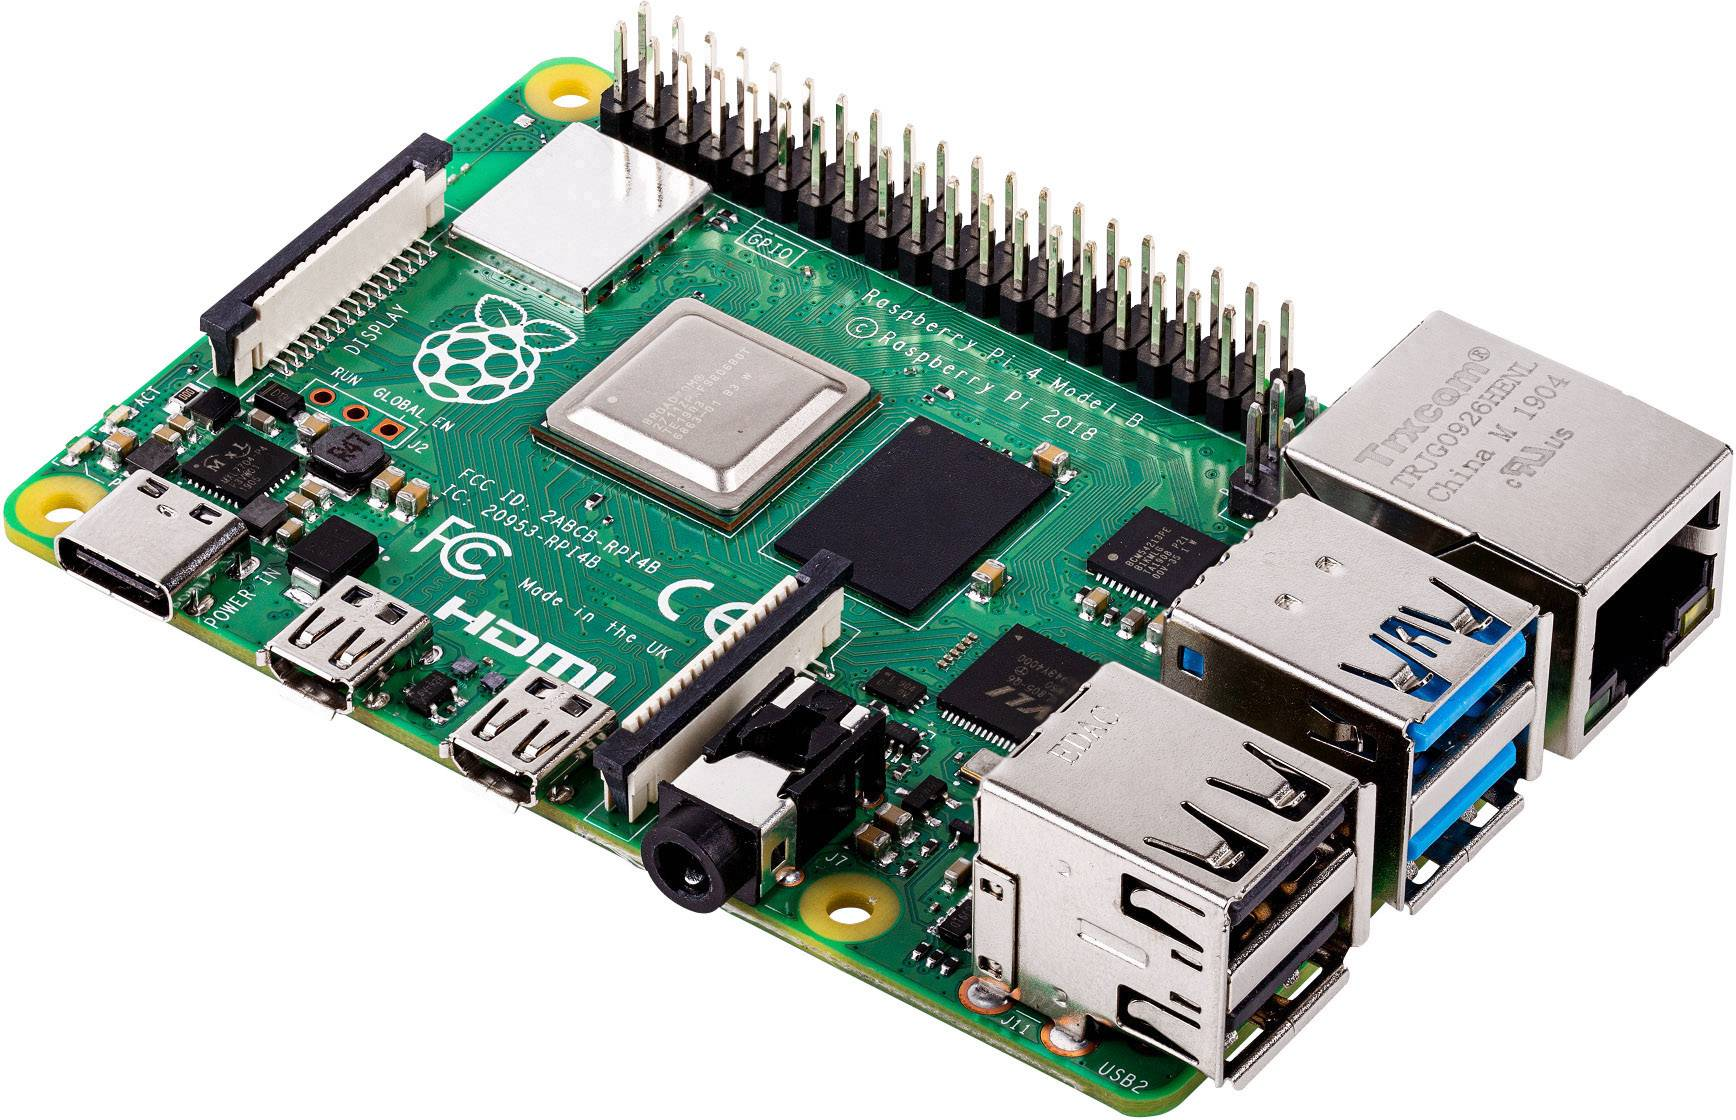
\includegraphics[height=3cm]{./01_Inhalte/07_RaspberryPi.jpg}
		\centering
		\caption{\acl{RasPi} 4}
	\end{figure}
\end{comment}

\subsection{\acl{RasPi} - Setup}
Um die Betriebssoftware auf die microSD-Karte zu schreiben, verwende ich Raspberry Pi Imager (Abbildung \ref{fig:RaspberryPiImager}). Als Systemsoftware würde ich empfehlen, Raspberry Pi OS (64 Bit) zu verwenden. Jedoch kann selbstverständlich auch ein anderes Betriebssystem bzw. die Lite/Full-Version davon benützt werden.

\begin{minipage}{0.5\textwidth}
	\begin{figure}[H]
		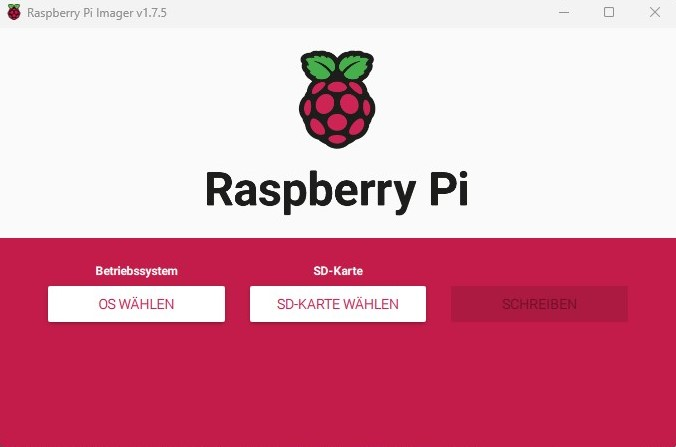
\includegraphics[height=5cm]{./01_Inhalte/08_Imager.jpg}
		\centering
		\caption{Raspberry Pi Imager}
		\label{fig:RaspberryPiImager}
	\end{figure}
\end{minipage}%
\begin{minipage}{0.5\textwidth}		
	\begin{figure}[H]
		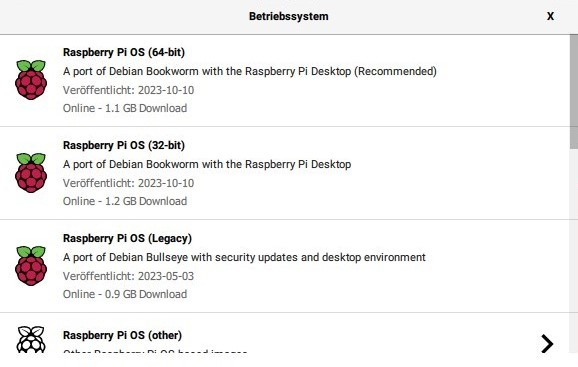
\includegraphics[height=5cm]{./01_Inhalte/08a_RaspberryPi_OS.jpg}
		\centering
		\caption{Raspberry Pi OS (64 Bit)}
		\label{fig:RaspberryPiOS}
	\end{figure}
\end{minipage}	
\\ \\
Nach Auswahl des Betriebssystems ist es ratsam noch unter den erweiterten Einstellung (Abbildung \ref{fig:ImagerOptionen}) einen Hostnamen zu vergeben und SSH zu aktivieren. Je nach Bedarf kann hier auch direkt eine WLAN-Verbindung eingerichtet werden. In diesem Fall werden für die SSH-Verbindung folgenden Zugangsdaten verwendet:


\begin{minipage}{0.5\textwidth}
	\begin{itemize}
		\item Benutzername: admin
		\item Passwort: Kennwort1
	\end{itemize}
\end{minipage}%
\begin{minipage}{0.5\textwidth}		
	\begin{figure}[H]
		\centering
		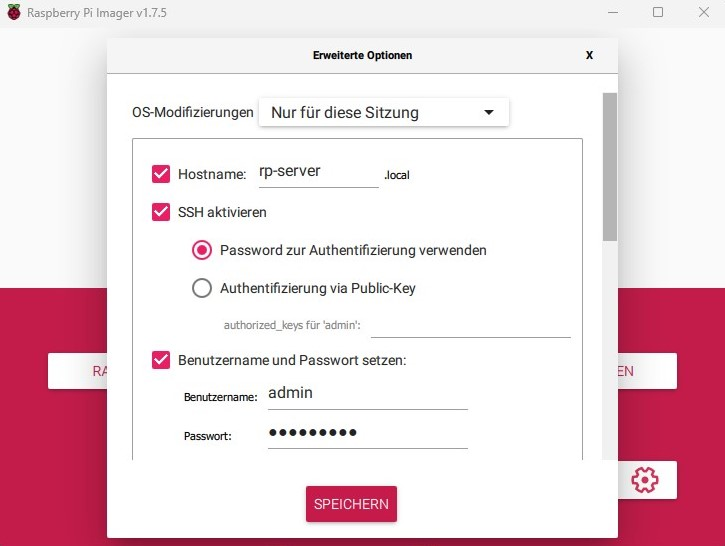
\includegraphics[width=6.8cm]{./01_Inhalte/08b_Imager_Optionen.jpg}
		\caption{Erweiterte Optionen}
		\label{fig:ImagerOptionen}
	\end{figure}
\end{minipage}	



Nach Abschluss des Schreibe- und Verifizierungsvorgangs kann die microSD-Karte entfernt und in den \ac{RasPi} eingesetzt werden. Sobald die IP-Adresse bekannt ist, ist es möglich, sich beispielsweise mit PuTTY über SSH mit dem \ac{RasPi} zu verbinden.

\begin{figure}[H]
	\centering
	\begin{subfigure}[t]{0.35\textwidth}
		\begin{adjustbox}{valign=c,center}
			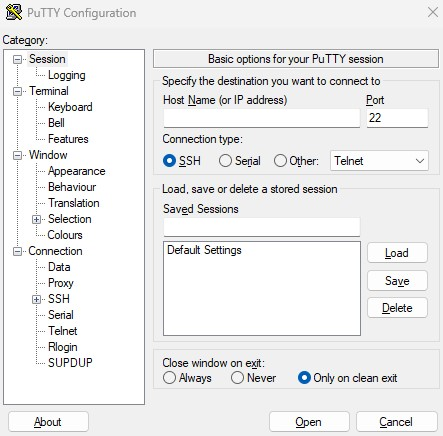
\includegraphics[width=\textwidth]{./01_Inhalte/08c_PuTTY.jpg}
		\end{adjustbox}
	\end{subfigure}
	\hfill
	\begin{subfigure}[t]{0.62\textwidth}
		\begin{adjustbox}{valign=c,center}
			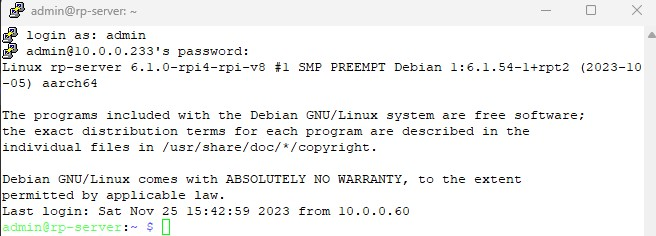
\includegraphics[width=\textwidth]{./01_Inhalte/08d_PuTTY.jpg}
		\end{adjustbox}
	\end{subfigure}
	\caption{PuTTY}
	\label{fig:PuTTY}
\end{figure}


\subsection{\ac{DBMS}}
Als \ac{DBMS} wird \textbf{MariadDB} verwendet. Zuerst sollte man die lokale Paketliste und alle installierten Softwarepakete aktualisieren. Falls man aufgefordert wird, fortzufahren, bestätige dies immer durch die Eingabe von ''Y''. Geben Sie die Befehle zudem immer einzeln ein.

\begin{Textfeld1}
	sudo apt update \\
	sudo apt upgrade
\end{Textfeld1}

Danach erfolgt die Installation des MariaDB-Servers durch Ausführen des folgenden Befehls:

\begin{Textfeld1}
	sudo apt install mariadb-server
\end{Textfeld1}

Nachdem die Installation abgeschlossen ist, führen wir die Grundkonfiguration mithilfe folgender Anweisung durch:

\begin{Textfeld1}
	sudo mysql\_secure\_installation
\end{Textfeld1}

Durch das Setup wie folgt durchgehen:

\begin{itemize}
	\item ''Enter current password for root'' = Bestätige mittels Enter-Taste (keine Eingabe).
	\item ''Switch to unix\_socket authentication?'' = n
	\item ''Change the root password?'' =  Y
	\begin{itemize}
		\item ''New password:'' = Kennwort1
		\item ''Re-enter new password:'' = Kennwort1
	\end{itemize}
	\item ''Remove anonymous users'' = Y
	\item ''Disallow root login remotely'' = Y
	\item ''Remove test database and access to it'' = Y
	\item ''Reload privilege tables now'' = Y
\end{itemize}

Um den Zugriff auf die \ac{DB} von anderen Rechnern zu ermöglichen, müssen wir noch den externen Zugriff aktivieren. Hierfür müssen wir folgendes File bearbeiten:

\begin{Textfeld1}
	sudo nano /etc/mysql/mariadb.conf.d/50-server.cnf
\end{Textfeld1}

Wir ändern die \textbf{bind-address} von 127.0.0.1 auf 0.0.0.0.

\begin{figure}[H]
	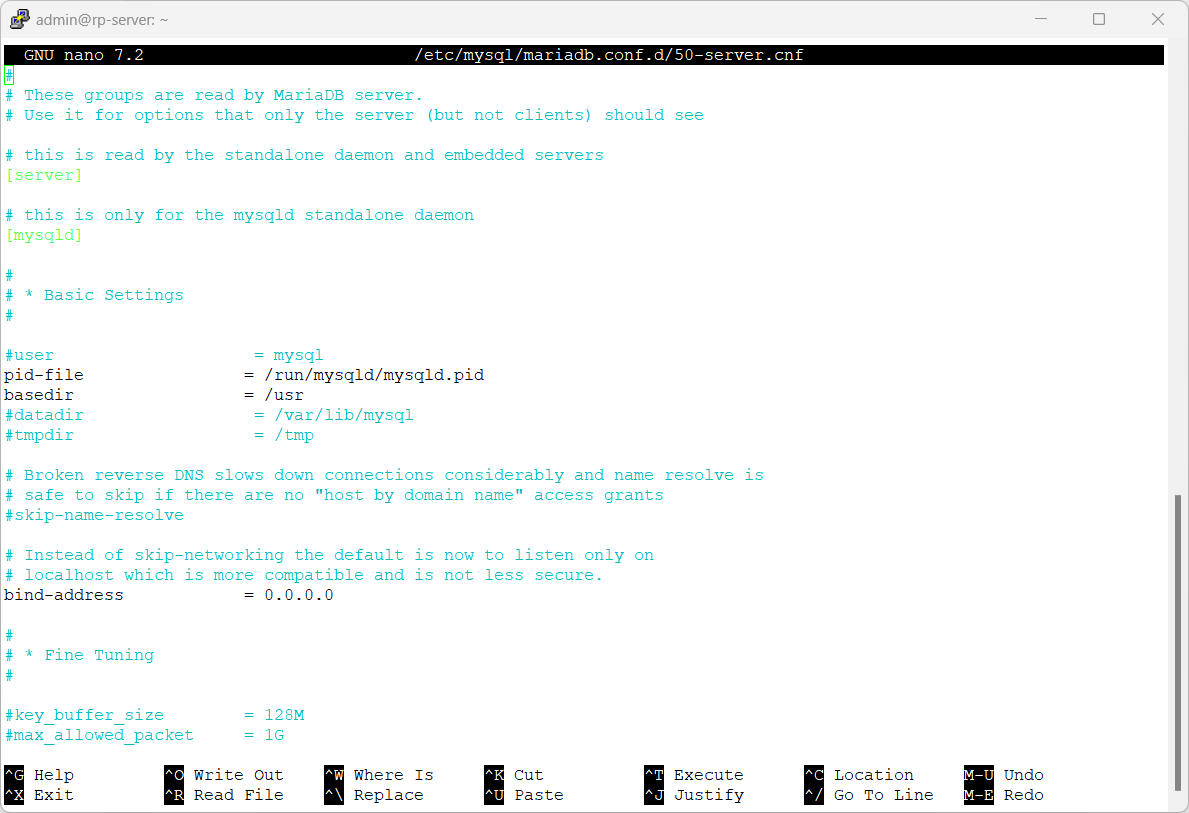
\includegraphics[scale=0.5]{./01_Inhalte/09_MariaDB_conf}
	\centering
	\caption{Externer Zugriff}
\end{figure}

Mit ''STR + O'' und dann ''Enter'' können wir die Änderungen speichern. Mittels der Tastenkombination ''STR + X'' verlassen wir danach den Editor.

\newpage
Im Anschluss müssen wir noch die Datenbank anlegen. Zu diesem Zweck verbinden wir uns mit dem Root-Account auf die \ac{DB}, in dem wir folgenden Befehl verwenden:

\begin{Textfeld1}
	sudo mysql -u root -p
\end{Textfeld1}

Daraufhin wird man aufgefordert das Passwort für den Root-User einzugeben, welches ''Kennwort1'' ist. Nun befinden wir uns in der MySQL-Shell, in welcher wir unsere SQL-Befehle ausführen können. Zuerst erstellen wir eine neue Datenbank mit folgender Anweisung:

\begin{Textfeld2}
	CREATE DATABASE Zeitmessung;
\end{Textfeld2}

Zusätzliche legen wir noch einen neuen Account an der nur Rechte über diese Datenbank besitzt.

\begin{itemize}
	\item Benutzername: mariadbclient
	\item Password: Kennwort1
\end{itemize}


Durch die Ausführung dieses Befehls wird der Benutzer erstellt:
\begin{Textfeld2}
	CREATE USER 'mariadbclient'@'\%' IDENTIFIED BY 'Kennwort1'; 
\end{Textfeld2}

Danach müssen wir diesem Benutzer noch Berechtigungen für die zuvor erstellte \ac{DB} erteilen:
\begin{Textfeld2}
	GRANT ALL PRIVILEGES ON Zeitmessung.* TO 'mariadbclient'@'\%'; 
\end{Textfeld2}

Zuletzt müssen wir noch die Berechtigungen neu laden:
\begin{Textfeld2}
	FLUSH PRIVILEGES;
\end{Textfeld2}

Um die MySQL-Shell zu verlassen und zur normalen Linux-Shell zurückzukehren, verwenden wir folgende Anweisung:

\begin{Textfeld2}
	exit;
\end{Textfeld2}

Es ist ratsam nach der Installation des Mariadb-Servers den \ac{RasPi} neu zu starten:
\begin{Textfeld1}
	sudo reboot
\end{Textfeld1}

Auf diese Weise haben wir erfolgreich das \ac{DBMS} installiert und müsse nun nur noch die benötigten Tabellen erstellten. Hierfür muss man lediglich die \ac{GUI} (Abschnitt \ref{sec:GUI}) einmalig starten und alle noch nicht vorhandenen Tabellen werden automatisch erzeugt. Dieser Schritt sollte jedoch erst nach Installation des MQTT-Brokers durchgeführt werden, um potenzielle Verbindungsfehler mit dem  Broker zu vermeiden.

\begin{figure}[H]
	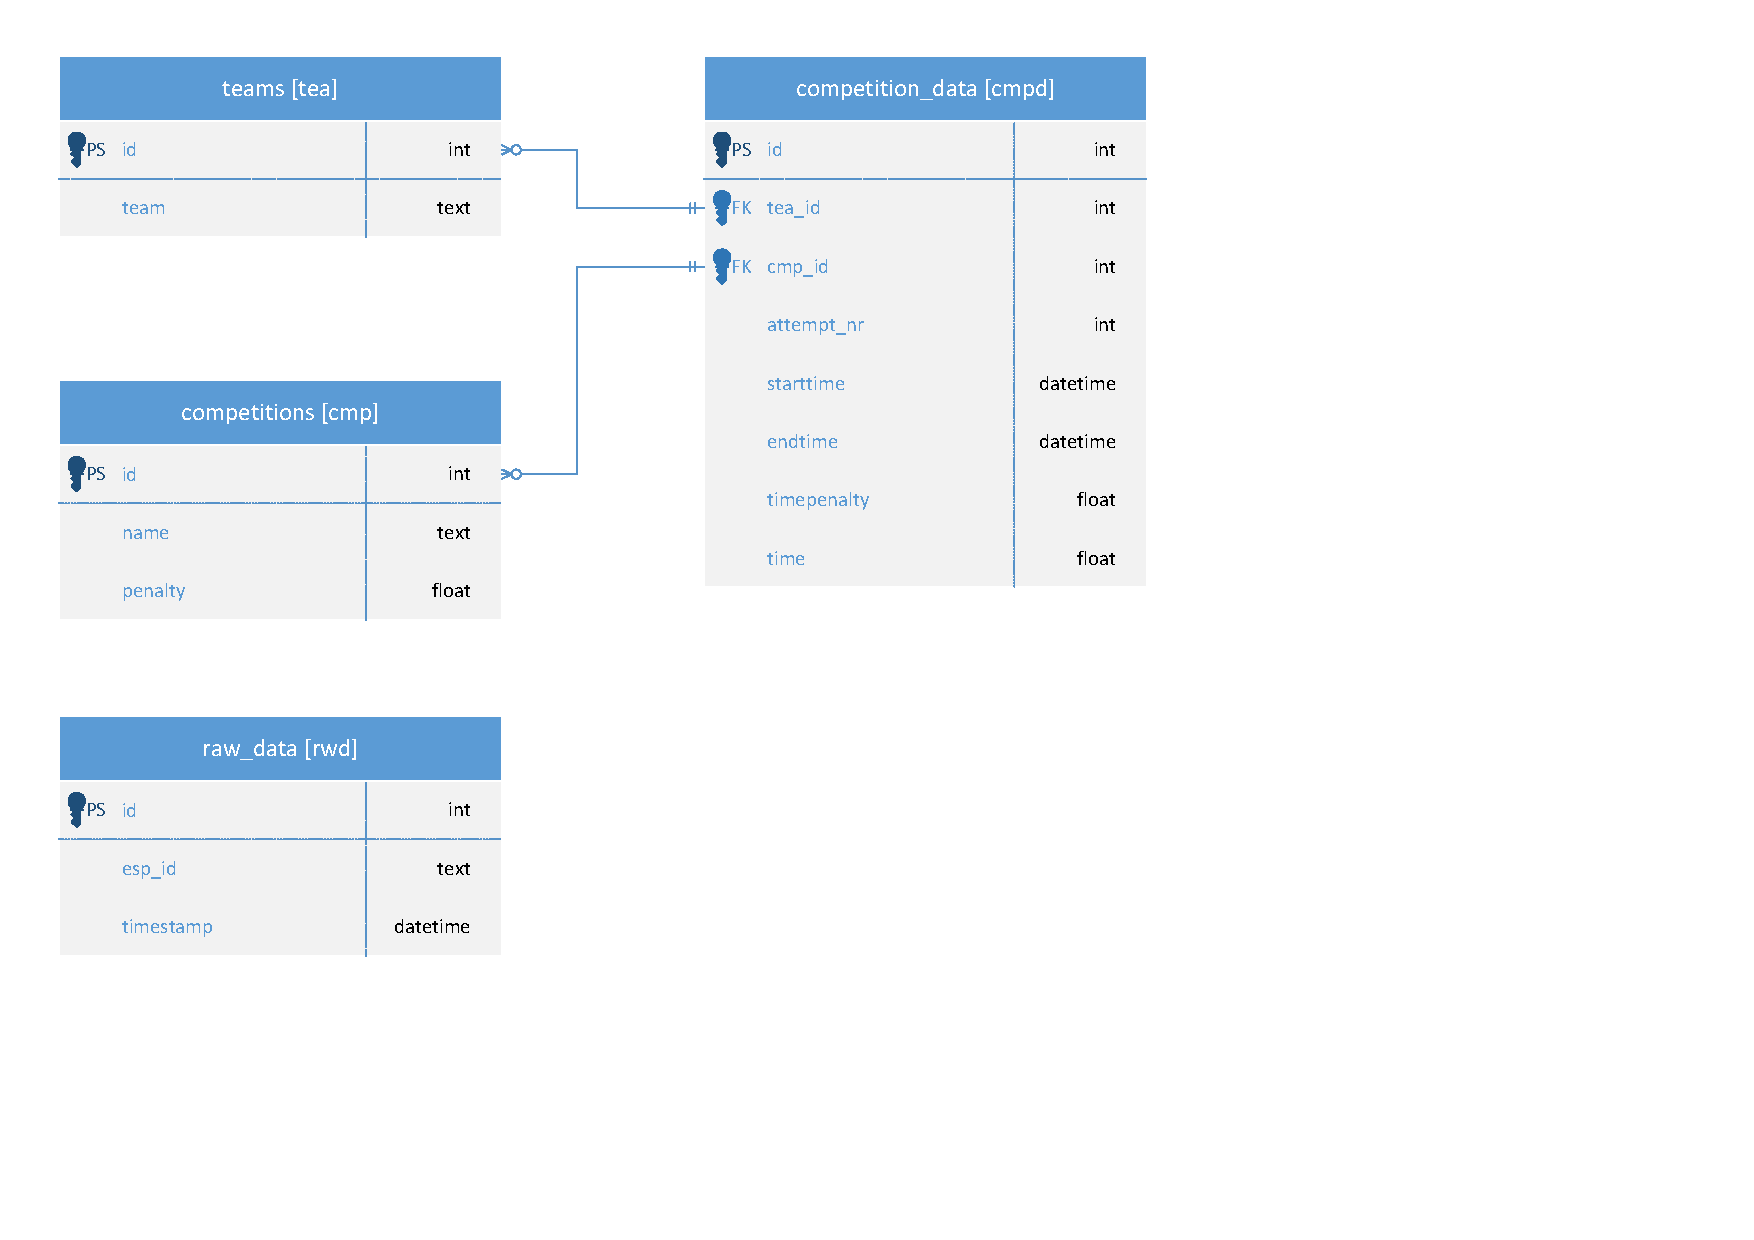
\includegraphics[width=0.65\textwidth]{./01_Inhalte/10_DB_Struktur.pdf}
	\centering
	\caption{\ac{DB}-Struktur}
\end{figure}


\subsubsection{PHPMyAdmin}
Zur leichteren Handhabung der MariaDB-Datenbank empfehle ich PHPMyAdmin zu installieren:
\begin{Textfeld1}
	sudo apt install phpmyadmin
\end{Textfeld1}
Falls man aufgefordert wird, fortzufahren, bestätige dies immer durch die Eingabe von ''Y''. Durch das Setup wie folgt durchgehen:
\begin{itemize}
	\item ''Web server to reconfigure automatically:'' = apache2 mit Leertaste auswählen und mit Enter bestätigen
	\item ''Configure database for phpmyadmin with dbconfig-common?'' = Yes mit Leertaste bestätigen
	\item ''MySQL application password for phpmyadmin:'' = ''Kennwort1'' mit Enter bestätigen
	\item ''Password confirmation:'' = ''Kennwort1'' mit Enter bestätigen
\end{itemize}
Somit wurde PHPMyAdmin erfolgreich installiert. Mittels der IP-Adresse des \ac{RasPi} und der Erweiterung ''/phpmyadmin'' kann lokal im Webbrowser auf die Anwendung zugegriffen werden (z.B.: 192.168.0.x/phpmyadmin). Als Benutzer würde ich empfehlen den Root-Account zu verwenden, da dieser Zugriffsrechte auf alle Datenbanken besitzt:
\begin{itemize}
	\item Benutzername: root
	\item Passwort: Kennwort1
\end{itemize} 


\subsection{MQTT Broker}
Zunächst installieren wir den MQTT-Broker. Wir verwenden in diesem Fall Mosquitto.
\begin{Textfeld1}
	sudo apt install mosquitto
\end{Textfeld1}

Anschließend stellen wir sicher das Mosquitto bei einem Neustart automatisch startet:
\begin{Textfeld1}
	sudo systemctl enable mosquitto
\end{Textfeld1}

Abschließend erstellen wir noch einen Benutzer für den MQTT-Broker:
\begin{itemize}
	\item Benutzername: mqttclient
	\item Password: Kennwort1
\end{itemize}
\begin{Textfeld1}
	sudo mosquitto\_passwd -c /etc/mosquitto/credentials mqttclient
\end{Textfeld1}

Daraufhin werden wir aufgefordert das Password einzugeben:
\begin{itemize}
	\item ''New password:'' = Kennwort1
	\item ''Re-enter new password:'' = Kennwort1
\end{itemize}

Hierdurch wird automatische eine Passwort-Datei erzeugt. Nun müssen wir Mosquitto noch konfigurieren:
\begin{Textfeld1}
	sudo nano /etc/mosquitto/conf.d/local.conf
\end{Textfeld1}

\newpage
In diese Konfigurations-Datei fügen wir noch folgende Zeilen ein:
\begin{figure}[H]
	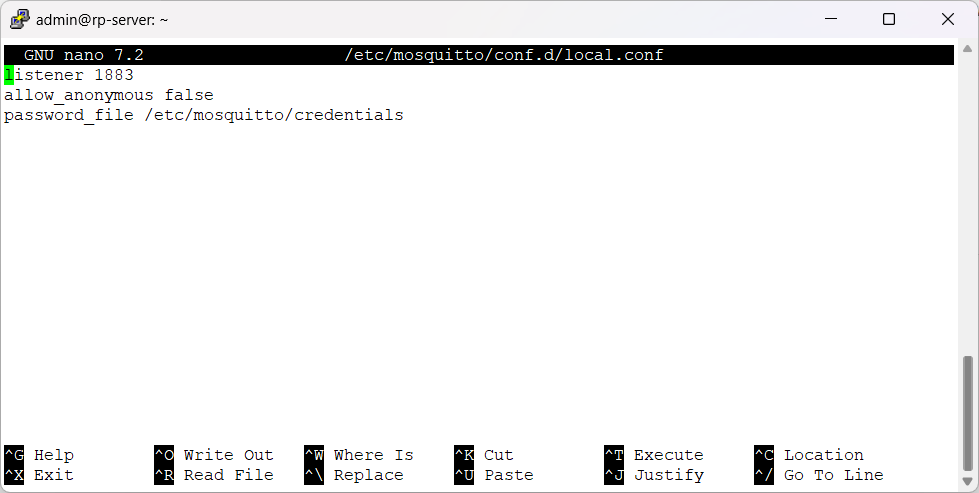
\includegraphics[width=0.9\textwidth]{./01_Inhalte/11_Mosquitto_conf}
	\centering
	\caption{Mosquitto Konfiguration}
\end{figure}

Mit ''STR + O'' und dann ''Enter'' können wir die Änderungen speichern. Mittels der Tastenkombination ''STR + X'' verlassen wir danach den Editor. Damit die eben erstellte Konfiguration wirksam wird starten wir Mosquitto neu:
\begin{Textfeld1}
	sudo systemctl restart mosquitto
\end{Textfeld1}

Somit haben wir den MQTT-Broker erfolgreich installiert und konfiguriert.

\begin{comment}
	\subsection{Webserver \& Services}
	Für die übersichtliche Darstellung der Ergebnisse der einzelnen Teams bzw. Challenges sowie des gesamten Bewerbs wurde ein Webserver konstruiert. Damit dieser funktioniert, müssen einige Dateien auf den \ac{RasPi} kopiert und Services hierfür aktiviert werden. Darüber hinaus verfügt das Service über eine Anwendung, welche alle Zeitstempel der Lichtschranke erfasst und speichert, unabhängig davon, ob sie verwendet werden. Hierfür muss der Ordner \textbf{01\_RP-Zeitmessung} auf das Homeverzeichnis des Benutzers ''admin'' (/home/admin) kopieren werden. Hierfür würde ich \textbf{WinSCP} empfehlen. Wird ein anderer Pfad gewünscht bzw. verwendet, muss man in den Dateien \textbf{startup\_script.sh} und \textbf{webserver.service}, welche sich im Verzeichnis \textbf{01\_RP-Zeitmessung} befinden, den Pfad anpassen, um den fehlerfreien Betrieb sicherzustellen. Bevor man jedoch den das Service aktiviert, muss man noch die Benutzerdaten im Python-Programm \textbf{app.py} im Verzeichnis \textbf{01\_RP-Zeitmessung} anpassen. Hierfür ist es ratsam, dies direkt in Visual Studio Code zu erledigen, bevor man den Ordner auf den \ac{RasPi} kopiert.
	\begin{lstlisting}[language=Python]
		# Database configuration
		DB_USER = "mariadbclient"       
		DB_PASSWORD = "Kennwort1"       
	\end{lstlisting}
	
	Zusätzlich muss man auch noch die Benutzerdaten im Programm \textbf{raw\_esp.py} im Ordner \textbf{01\_RP-Zeitmessung} modifizieren:
	\begin{lstlisting}[language=Python]
		# MQTT configuration
		MQTT_USER = "mqttclient"        
		MQTT_PASSWORD = "Kennwort1"    
		
		# Database configuration
		DB_USER = "mariadbclient"       
		DB_PASSWORD = "Kennwort1"     
	\end{lstlisting}
	
	Daraufhin kopieren wir mittels WinSCP den Ordner \textbf{01\_RP-Zeitmessung} auf den \ac{RasPi} in das Verzeichnis \textbf{/home/admin}. 
	\begin{figure}[H]
		\centering
		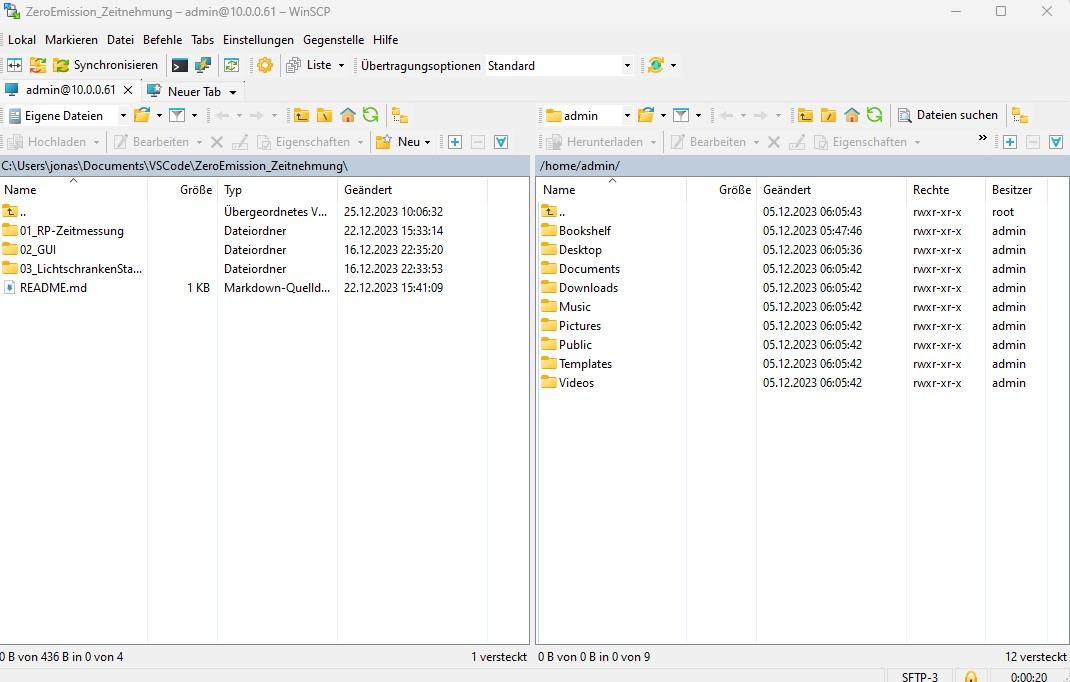
\includegraphics[width=0.85\textwidth]{./01_Inhalte/12_WinSCP}
		\caption{WinSCP}
	\end{figure}
	
	Danach müssen wir noch die Service-Datei in den richtigen Ordner verschieben.
	\begin{Textfeld1}
		sudo mv /home/admin/01\_RP-Zeitmessung/webserver.service /etc/systemd/system
	\end{Textfeld1}
	
	Anschließend müssen wir noch Ausführungsrechte rekursiv für das gesamte Verzeichnis erteilen:
	\begin{Textfeld1}
		chmod -R +x /home/admin/01\_RP-Zeitmessung
	\end{Textfeld1}
	
	Nachher laden wir mit dem folgenden Befehl den Systemd-Deamon neu :
	\begin{Textfeld1}
		sudo systemctl daemon-reload
	\end{Textfeld1}
	
	Als Nächstes starten wir das Service und aktivieren den automatischen Start bei Systemstart:
	\begin{Textfeld1}
		sudo systemctl start webserver \\
		sudo systemctl enable webserver
	\end{Textfeld1}
	
	Somit wurde der Webserver erfolgreich aktiviert. Man kann nun auf die Anwendung zugreifen, indem man die IP-Adresse des \ac{RasPi} und die Erweiterung '':5000'' in seinem Webbrowser eingibt. Zum Beispiel: \textbf{''192.168.0.x:5000''}.
\end{comment}


\subsection{Webserver \& Services}
Für die übersichtliche Darstellung der Ergebnisse der einzelnen Teams bzw. Challenges sowie des gesamten Bewerbs wurde ein Webserver konstruiert. Damit dieser funktioniert, müssen einige Dateien auf den \ac{RasPi} kopiert und der Apache2-Webserver hierfür konfiguriert werden. Darüber hinaus verfügt das Service über eine Anwendung, welche alle Zeitstempel der Lichtschranken erfasst und speichert, unabhängig davon, ob sie verwendet werden. Hierfür muss der Ordner \textbf{01\_RP-Zeitmessung} in das Verzeichnis \textbf{/var/www} kopieren werden. Hierfür würde ich \textbf{WinSCP} empfehlen. Bevor man jedoch den den Ordner auf den \ac{RasPi} kopiert, muss man noch die Benutzerdaten im Python-Programm \textbf{app.py} im Verzeichnis \textbf{01\_RP-Zeitmessung} anpassen. 
\newpage
Hierfür ist es ratsam, dies direkt in Visual Studio Code zu erledigen.

\begin{lstlisting}[language=Python]
	# MQTT configuration
	MQTT_USER = "mqttclient"        
	MQTT_PASSWORD = "Kennwort1"    
	
	# Database configuration
	DB_USER = "mariadbclient"       
	DB_PASSWORD = "Kennwort1"     
\end{lstlisting}

Danach kann man mit WinSCP den Ordner \textbf{01\_RP-Zeitmessung} auf den \ac{RasPi} ins Verzeichnis \textbf{''/home/admin''} kopieren, da dem Benutzer ''admin'' die Rechte fehlen für das Verzeichnis \textbf{''/var/www''}. Dies kann man direkt mit ''Drag and Drop'' durchführen.
\begin{figure}[H]
	\centering
	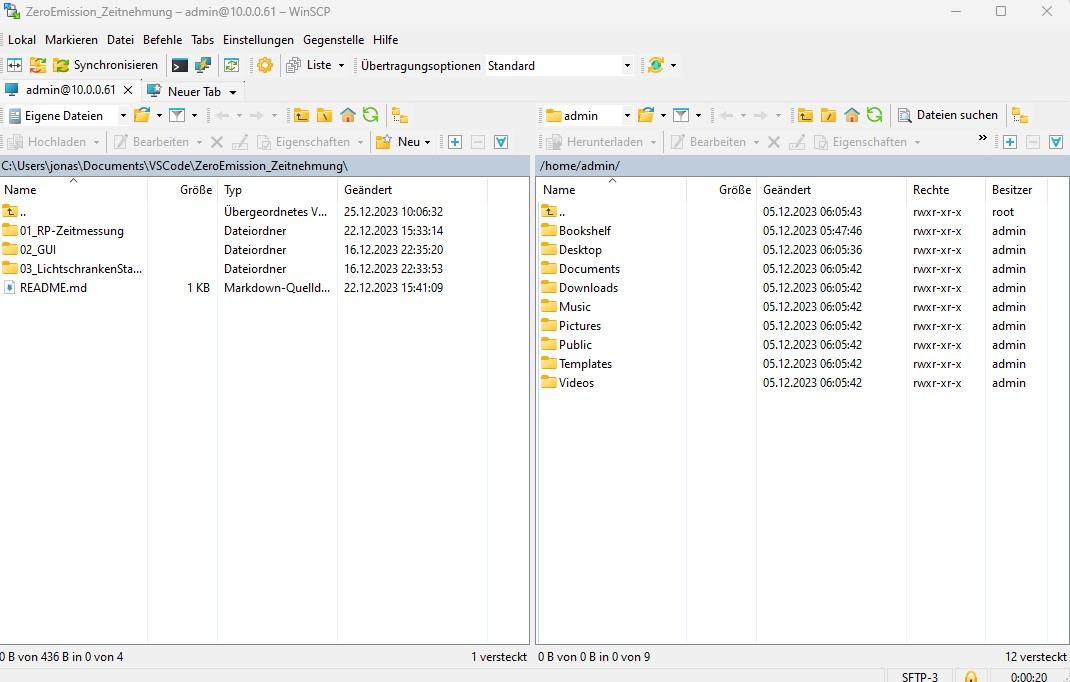
\includegraphics[width=0.85\textwidth]{./01_Inhalte/12_WinSCP}
	\caption{WinSCP}
\end{figure}

Folglich verschieben wir den Ordner mit Root-Rechten in das richtige Verzeichnis und ändern die Gruppenzugehörigkeit des Ordners. Die Befehle immer einzeln eingeben.
\begin{Textfeld1}
	sudo mv /home/admin/01\_RP-Zeitmessung /var/www \\
	sudo chown -R admin:www-data /var/www/01\_RP-Zeitmessung
\end{Textfeld1}

Anschließend muss man die Serverkonfigurations-Datei noch in das richtige Verzeichnis verschieben.
\begin{Textfeld1}
	sudo mv /var/www/01\_RP-Zeitmessung/webserver.conf /etc/apache2/sites-available
\end{Textfeld1}

Zudem muss man \textbf{mod\_wsgi} installieren und aktivieren:
\begin{Textfeld1}
	sudo apt install libapache2-mod-wsgi-py3 \\
	sudo a2enmod wsgi
\end{Textfeld1}

Darauf deaktivieren wir die Standartkonfiguration und aktivieren unsere Konfiguration:
\begin{Textfeld1}
	sudo a2dissite 000-default \\
	sudo a2ensite webserver
\end{Textfeld1}

Im Anschluss starten wir den Apache2-Server neu:
\begin{Textfeld1}
	sudo systemctl restart apache2
\end{Textfeld1}


\subsection{Implementierungsschritte}
Darüber hinaus ist es notwendig, die Teams und Herausforderungen manuell einzutragen. Dies kann auf zwei Arten erfolgen: entweder über phpMyAdmin für eine benutzerfreundliche Oberfläche oder direkt im Terminal. Um die Daten im Terminal einzufügen, beginnt man zunächst mit der Verbindung zur Datenbank:

\begin{Textfeld1}
	sudo mysql -u root -p
\end{Textfeld1}
Daraufhin wird man aufgefordert das Passwort für den Root-User einzugeben, welches ''Kennwort1'' ist. Danach wählen wir die Datenbank aus:

\begin{Textfeld2}
	USE Zeitmessung;
\end{Textfeld2}

Danach können wir schon die Teams eintragen:

\begin{Textfeld2}
	INSERT INTO teams (name) VALUES ('Team 1'), ('Team 2'), ('Team 3');
\end{Textfeld2}

Beziehungsweise die Challenges:
\begin{Textfeld2}
	INSERT INTO challenges (name,penalty) VALUES ('Challenge 1', 1.0), ('Challenge 2', 2.0);
\end{Textfeld2}

Mit folgenden Befehl kann man die MySQL-Shell verlassen:
\begin{Textfeld2}
	exit;
\end{Textfeld2}

Des Weiteren empfehle ich für den \ac{RasPi} eine statische IP-Adresse zu vergeben, welche im \ac{DHCP}-Server eingetragen werden muss.

\subsection{Allgemeine Befehle}
Zum Herunterfahren des \ac{RasPi} kann man diesen Befehl verwenden:
\begin{Textfeld1}
	sudo shutdown -P now
\end{Textfeld1}

Wenn ma überprüfen möchte, ob ein gewisses Service (z.B. MariaDB, Mosquitto) läuft, kann dies mit folgender Anweisung erfolgen:
\begin{Textfeld1}
	sudo systemctl status service\_name
\end{Textfeld1}

Möchte man ein Service stoppen bzw. starten, wird dieser Befehl verwendet:
\begin{Textfeld1}
	sudo systemctl stop service\_name \\
	sudo systemctl start service\_name
\end{Textfeld1}

Um das Service automatische bei Systemstart zu starten bzw. diesen Vorgang zu deaktivieren verwendet man:
\begin{Textfeld1}
	sudo systemctl enable service\_name \\
	sudo systemctl disable service\_name
\end{Textfeld1}

